\section{Instruction Set Architecture}
\frame{
\frametitle{\secname}
\begin{itemize}
    \item CPU Programs $=$ lots of instructions that the CPU steps through to execute
    \item ISA is how the CPU interprets those instructions.
    \item Examples: x86, RISC-V etc.
    \item There are \textbf{a lot} of instructions.
\end{itemize}
}

\section{x86 ISA}
\frame{
\frametitle{\secname}
\centering
\begin{figure}
    \centering
    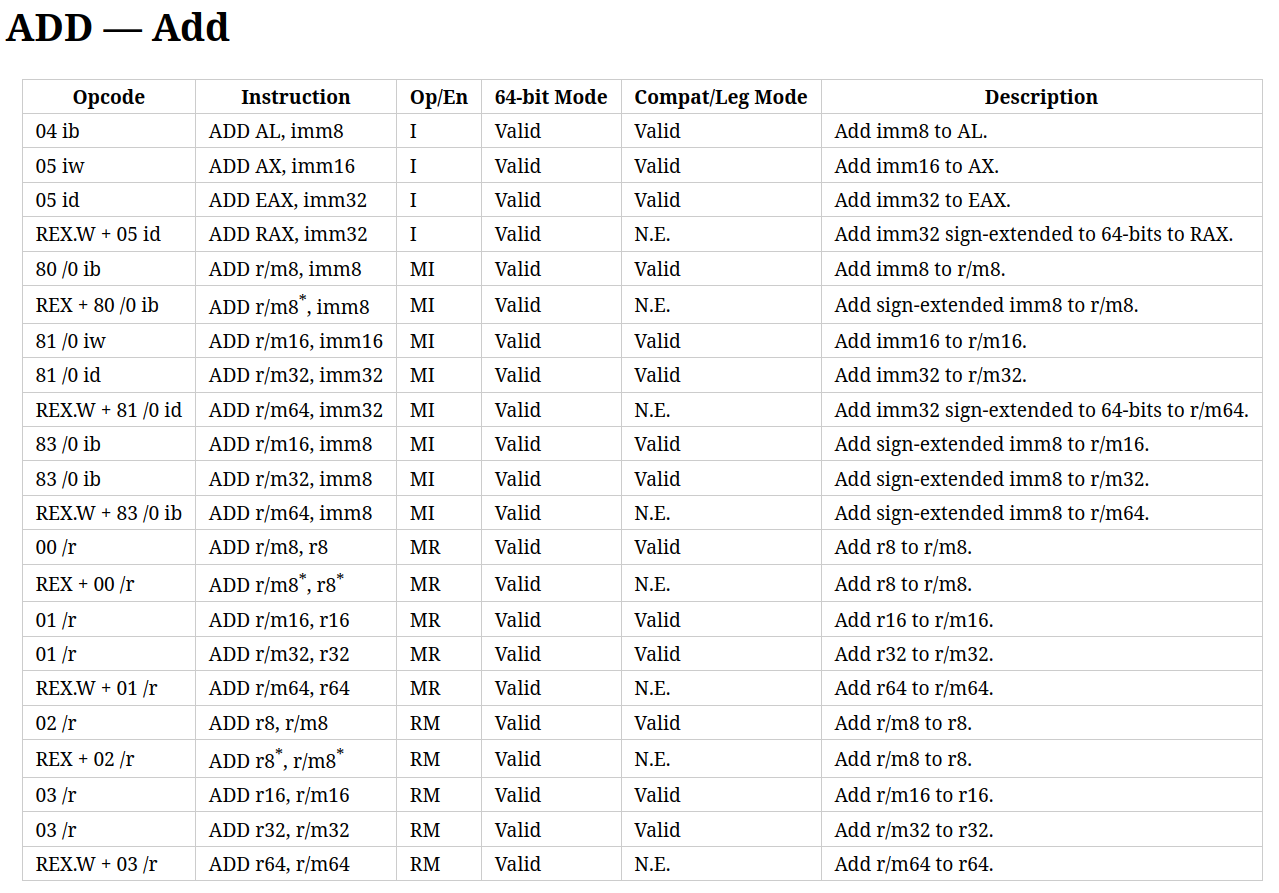
\includegraphics[width=0.8\linewidth]{slides/knotd/add.png}
\end{figure}
}

\section{x86 ISA}
\frame{
\frametitle{\secname}
\centering
\begin{figure}
    \centering
    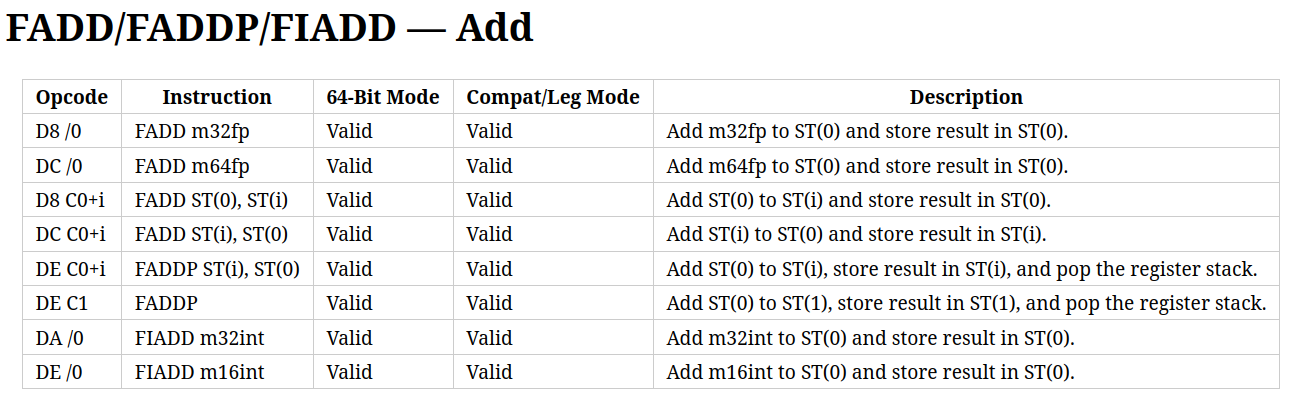
\includegraphics[width=0.7\linewidth]{slides//knotd/fadd.png}
    
    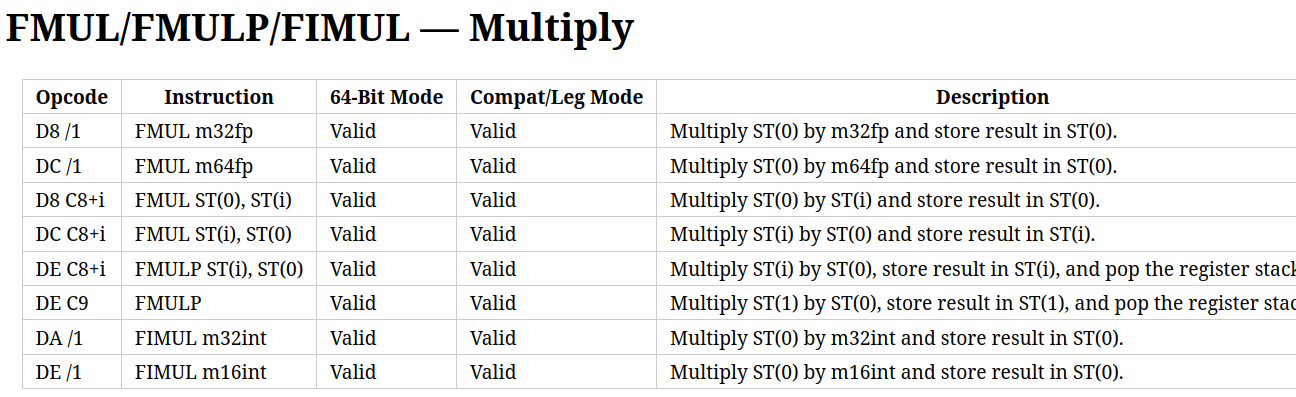
\includegraphics[width=0.7\linewidth]{slides//knotd/fmul.png}
\end{figure}
}

\section{x86 ISA}
\frame{
\frametitle{\secname}
\centering
\begin{figure}
    \centering
    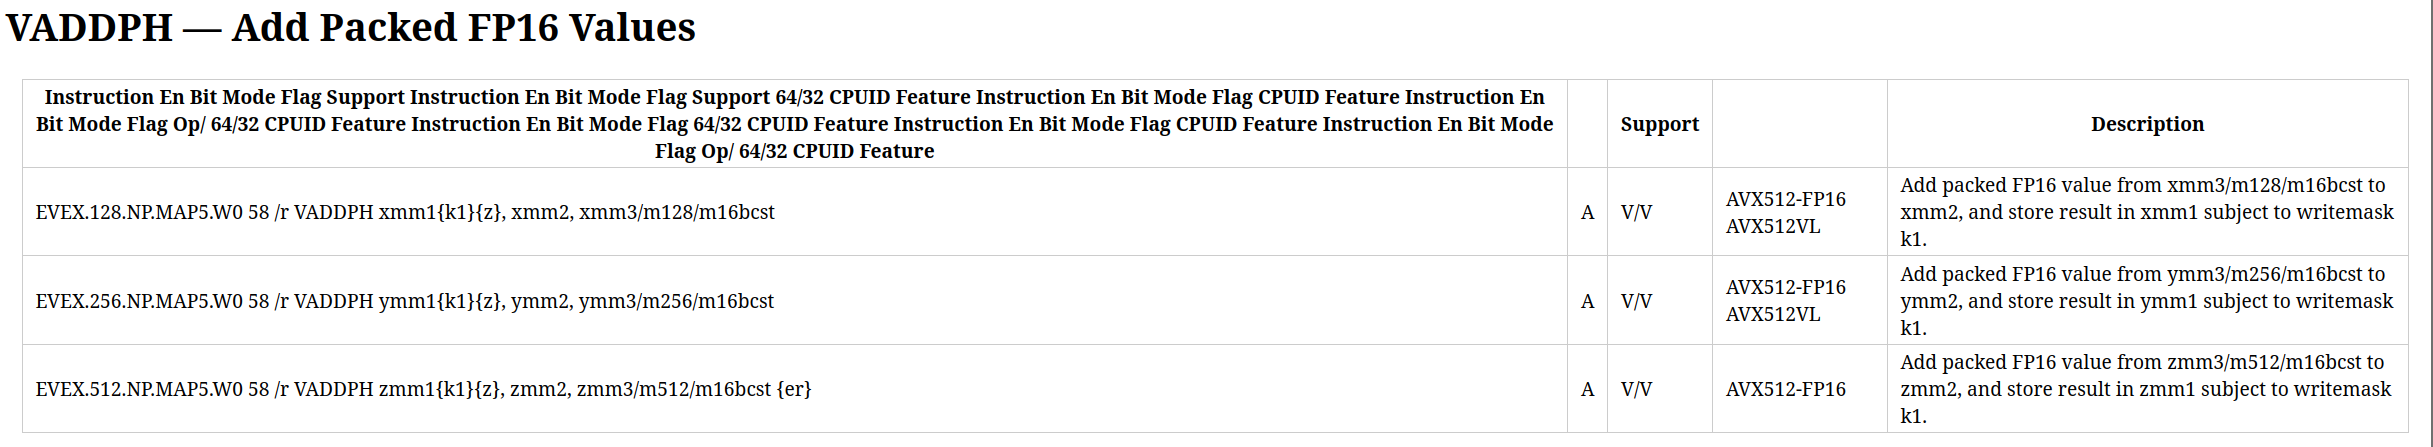
\includegraphics[width=1\linewidth]{slides//knotd/vaddph.png}

    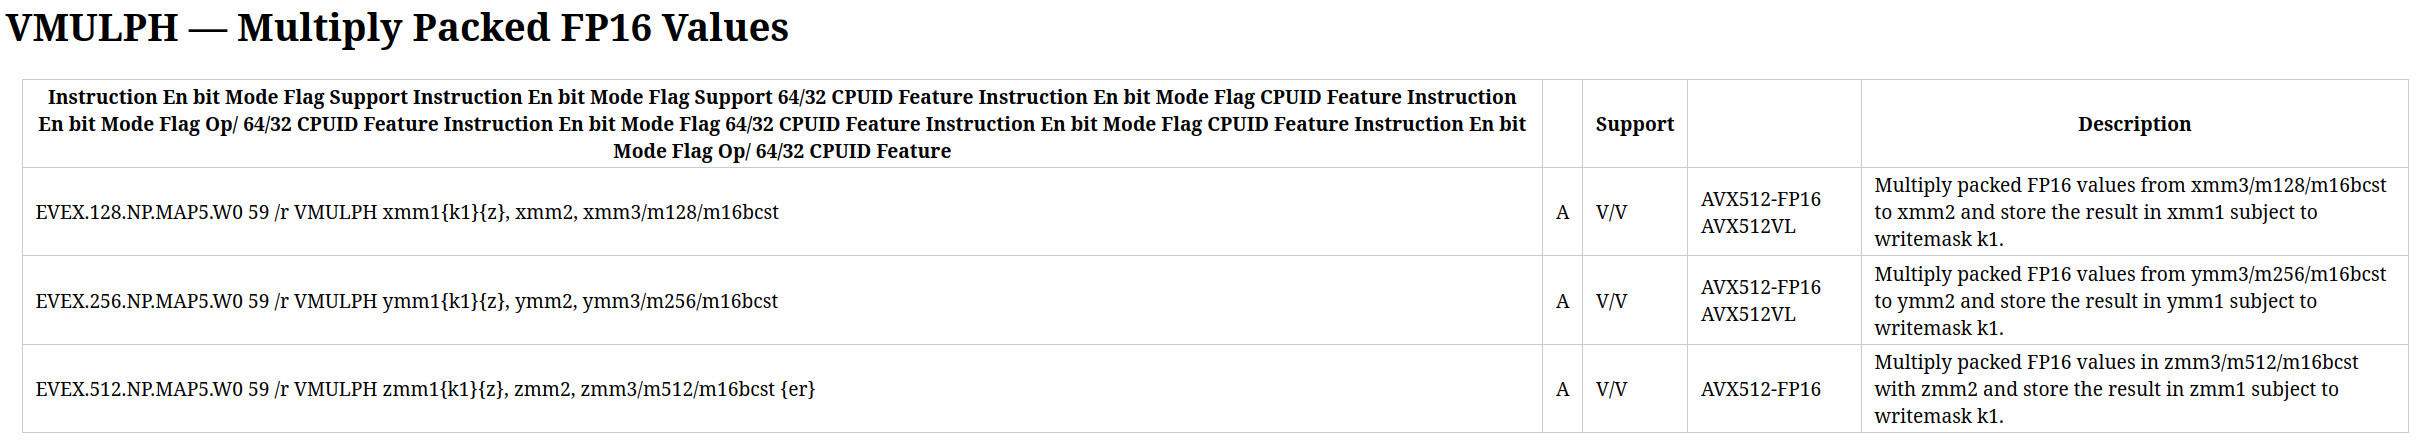
\includegraphics[width=1\linewidth]{slides//knotd/vmulph.png}
\end{figure}
}

\section{x86 ISA}
\frame{
\frametitle{\secname}
\centering
\begin{figure}
    \centering
    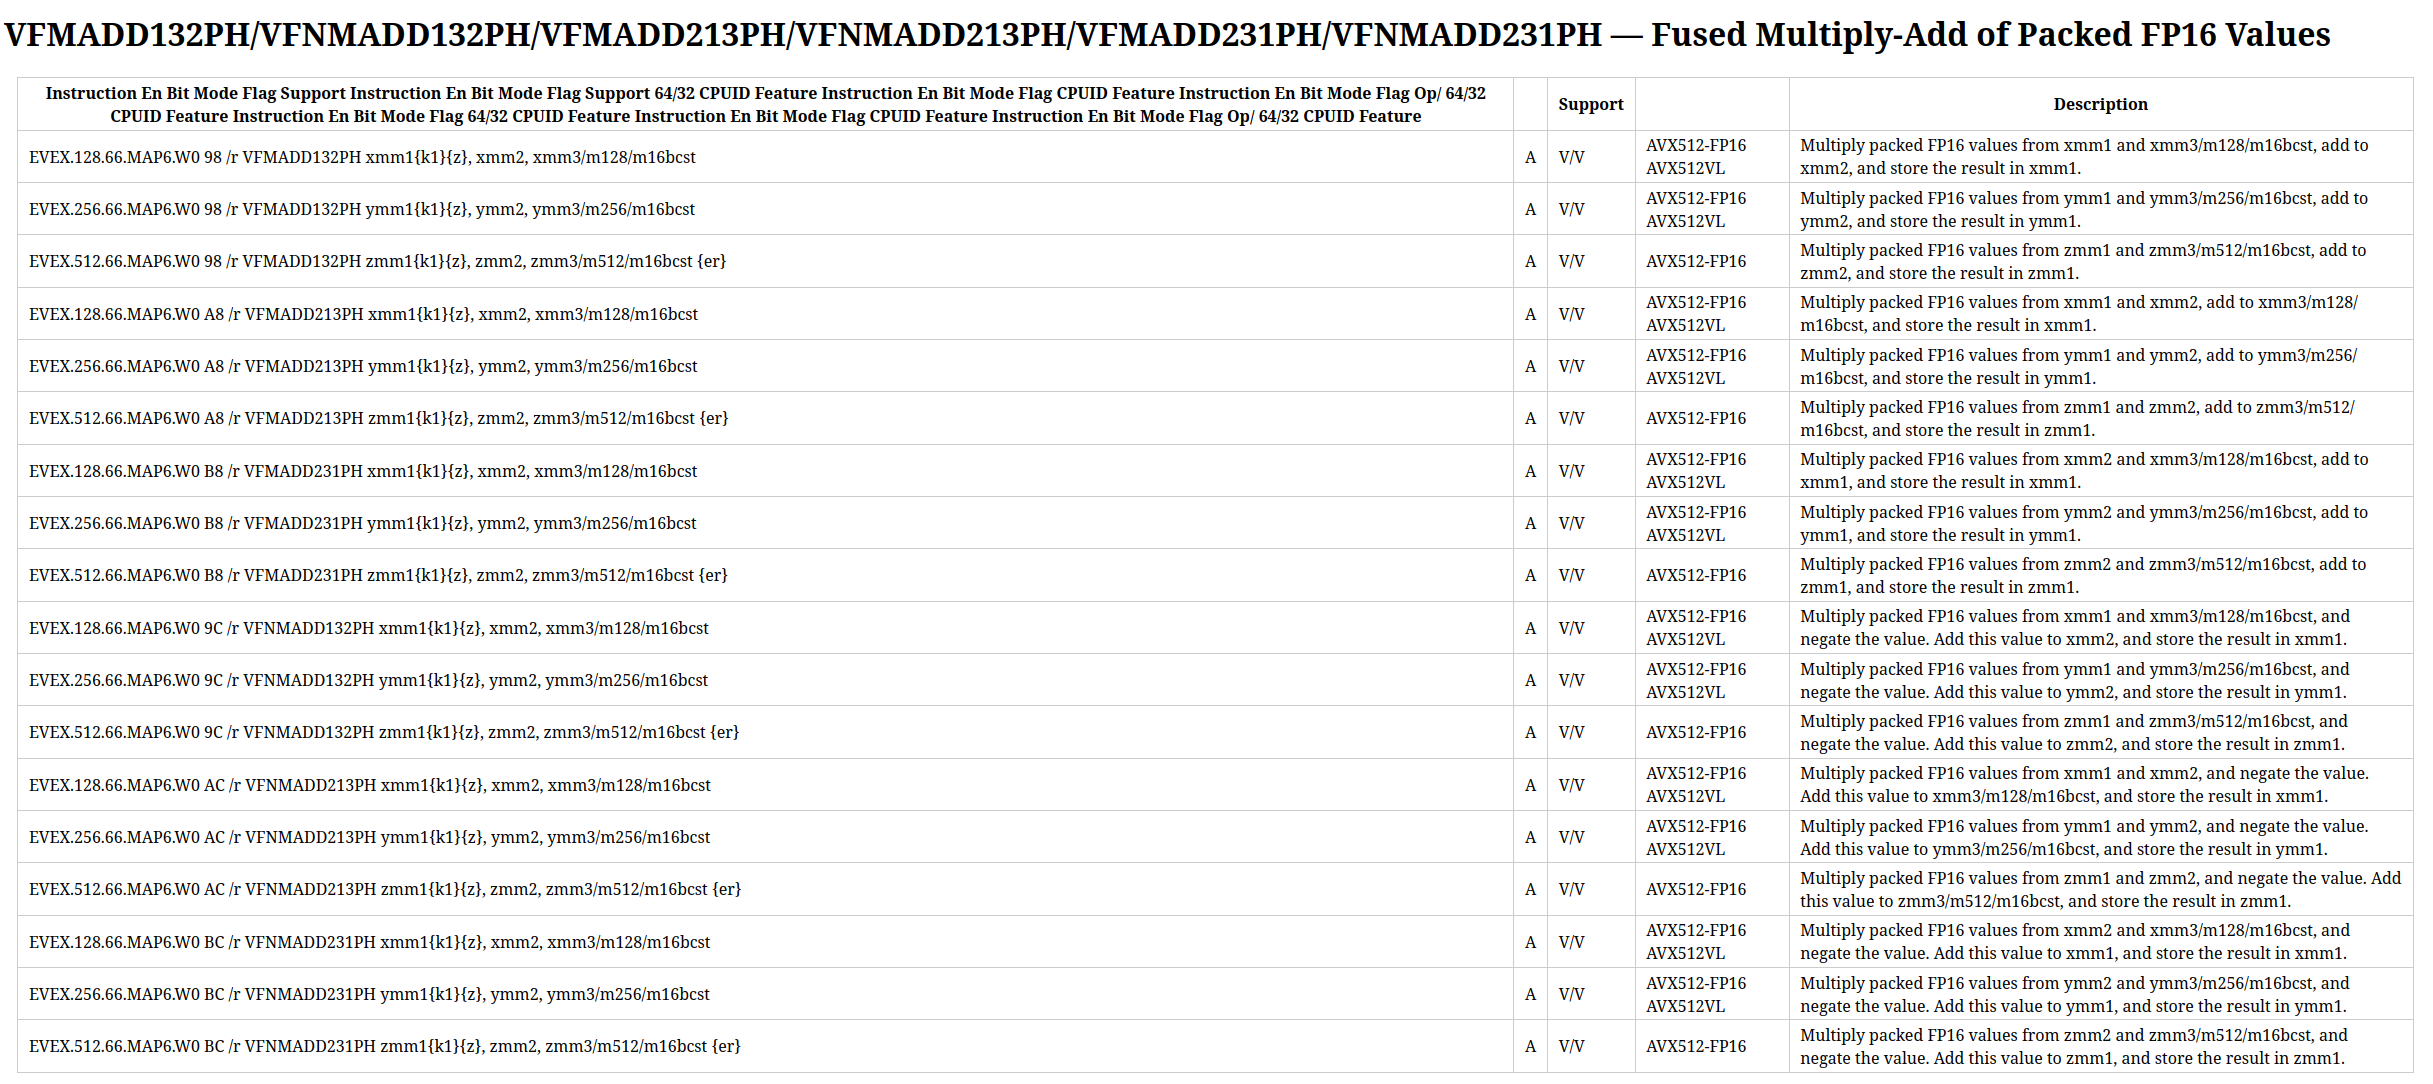
\includegraphics[width=1\linewidth]{slides//knotd/vfnmadd.png}
\end{figure}
}

\section{x86 ISA}
\frame{
\frametitle{\secname}
\centering
\begin{figure}
    \centering
    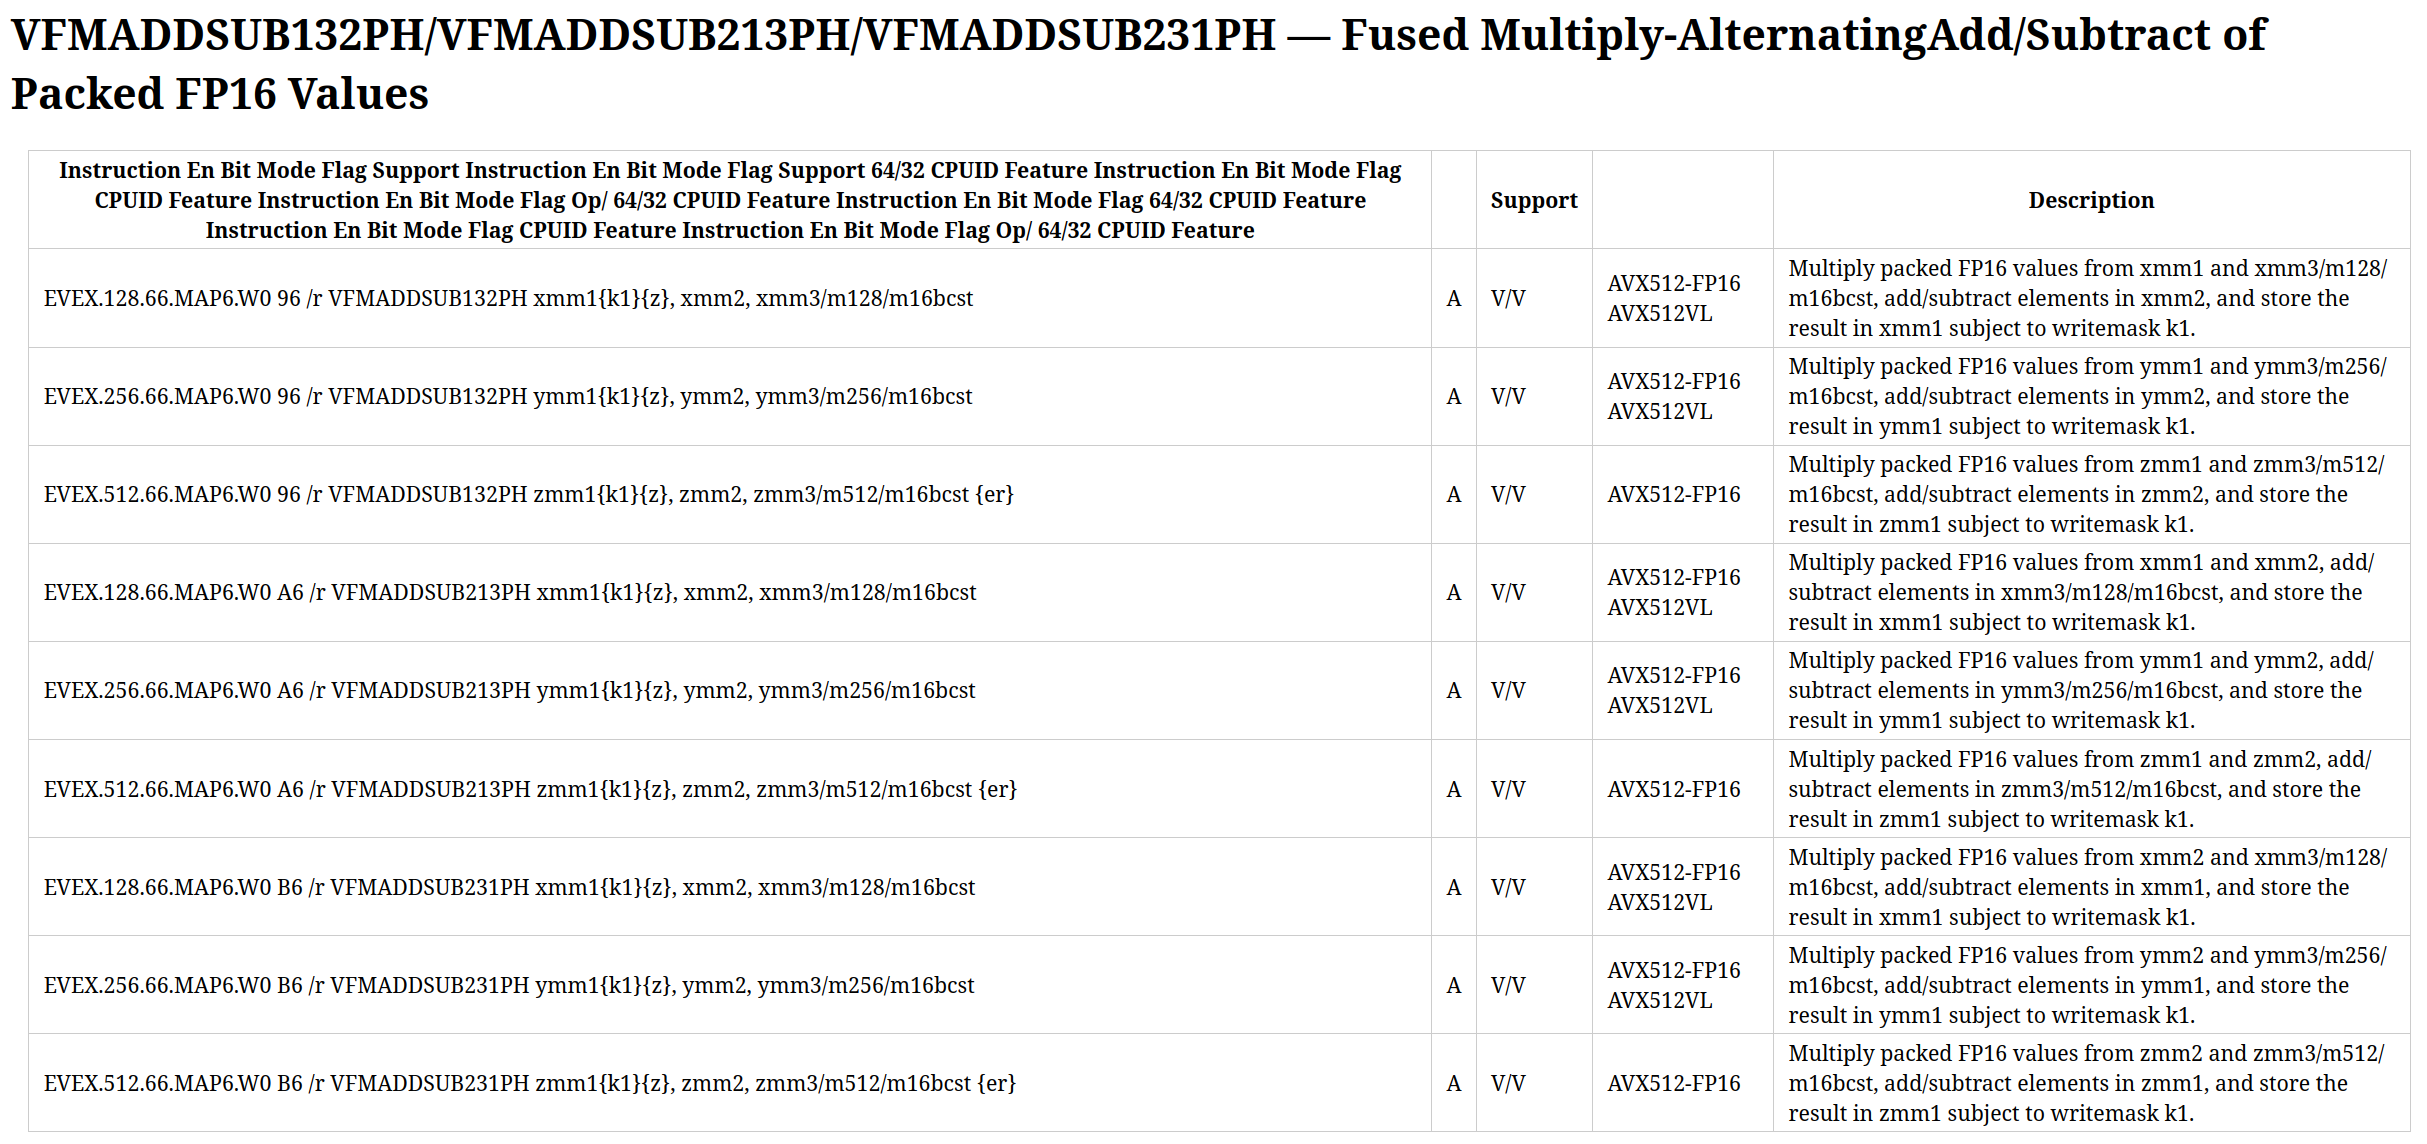
\includegraphics[width=1\linewidth]{slides//knotd/vfmaddsub.png}
\end{figure}
}

\section{x86 ISA}
\frame{
\frametitle{\secname}
\centering
\begin{figure}
    \centering
    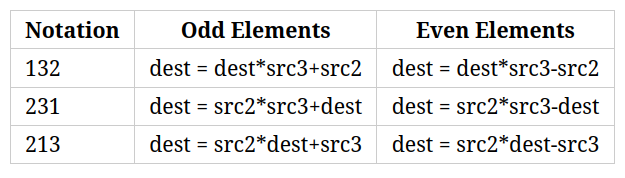
\includegraphics[width=1\linewidth]{slides//knotd/123-213-231.png}
\end{figure}
}

\section{KNOTD}
\frame{
\frametitle{\secname}
\centering
\includesvg[width=0.8\textwidth]{slides/knotd/x86_sdm_knotd}


\includegraphics[width=0.8\linewidth]{slides//knotd/rfurryirl_comment.png}

}
